%! TeX program = xelatex
\documentclass[../main.tex]{subfiles}

\begin{document}
\makelectureweek{6}{Week 6}

\section{Linear approximation}

\begin{mdframed}[style=withref]
  Let \(f(x)\) be a function and let \(a\) be a constant. A linear function \(L(x)\), defined by
  \[
    L(x) = {f'(a) (x - a) + f(a)}
  \]
  is called the {linear approximation} of \(f(x)\) near the point \((a, f(a))\). Sometimes, we also say \(L(x)\) is the linear approximation of \(f(x)\) at \(a\).

  \textbook{\stewart{254}{\fbox{1}}}
\end{mdframed}
\vspace{1in}

\begin{example}
  Approximate \(\sqrt{2}\) by linearizing \(\sqrt{x}\) at \(1\).
\end{example}
\vfill{}

\begin{example}
  Is it better to approximate \(\sqrt{2}\) by linearizing \(\sqrt{x}\) at \(1\) or at \(3\)? Can you explain this graphically?
\end{example}

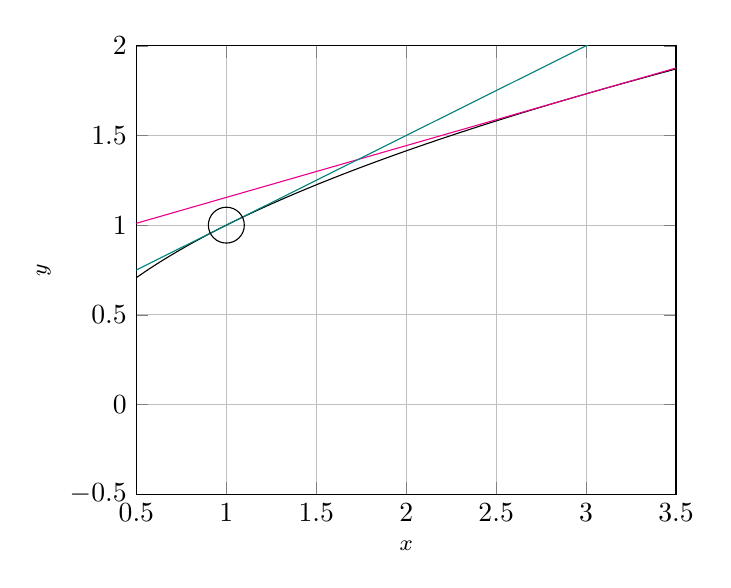
\begin{tikzpicture}
  \begin{axis}[
    xlabel={\footnotesize \(x\)},
    ylabel={\footnotesize \(y\)},
    % width={5in},
    xmin={0.5},
    xmax={3.5},
    ymin={-0.5},
    ymax={2},
    % xlabel style={at={(ticklabel* cs:1)}, anchor=west},
    % ylabel style={at={(ticklabel* cs:1)}, anchor=south},
    grid=both,
    ]
    \addplot[domain=0:5, no markers, smooth, samples=1000]{sqrt(x)};
    \addplot[domain=0:5, no markers, smooth, samples=1000, magenta]{sqrt(3) + 1/(2*sqrt(3))*(x-3)};
    \addplot[domain=0:5, no markers, smooth, samples=1000, teal]{1 + 1/2*(x-1)};
    \node[below left] at (axis cs:5,{sqrt(5)}) {\footnotesize \(\sqrt{x}\)};
    \draw (axis cs:1,1) circle (0.1);
  \end{axis}
\end{tikzpicture}

\clearpage

\begin{example}
  Approximate \(\sin(3)\).

  \bigskip
  \textbf{Step 1}. \emph{What} function \(f(x)\) should we linearize to approximate \(\sin(3)\)?
  \vspace{1.5in}

  \textbf{Step 2}. \emph{Where} should we linearize \(f(x)\) to approximate \(\sin(3)\)?
  \vspace{1.5in}

  \textbf{Step 3}. Linearize \(f(x)\) and find the answer.
  \vspace{2in}
\end{example}

% \hrule
% \textbf{Clarification of terminology.} Let \(f\) be a function and let \(a\) be a constant.
%
% When we say ``the tangent line of \(f(x)\) at \(x=a\),'' we mean
% \vfill
%
% When we say ``linearize \(f(x)\) at \(x=a\),'' we mean
% \vfill
%
% When we say ``find the linear approximation of \(f(a)\),'' we mean
% \vfill
%
\clearpage

\section{Exponential Growth and Decay}
Consider a special type of equation
\begin{equation} \label{eq:exp-de}
  \frac{dy}{dt} = ky,
\end{equation}
where 
\begin{itemize}
  \item \(k\) is {a constant}
    \bigskip

  \item \(y\) is {a function of \(t\)}
\end{itemize}
\vspace{1in}

Suppose \(k = 1\). Can you guess a solution to \(\frac{dy}{dt} = y\)?
\vspace{1in}

What does Equation~\eqref{eq:exp-de} tell us 
\vfill

\clearpage

\begin{mdframed}[style=withref]
  The only solutions to \(\frac{dy}{dt} = ky\) are 
  \begin{equation} \label{eq:exp-model}
    {y(t) = y(0) e^{kt}.}
  \end{equation}

  \textbook{\stewart{239}{\fbox{2} Theorem}}
\end{mdframed}

\textbf{Terminologies}. 
\begin{itemize}

\item The constant \(k\) is called
  \bigskip

\item The value \(y(0)\) is called the 
  \bigskip
\end{itemize}

Explore Equation~\eqref{eq:exp-model} using GeoGebra: \url{https://www.geogebra.org/calculator/rjdp3zxd}

\bigskip

\begin{example}
  Let's develop a mathematical model for the world population since 1950. 
  Assume that the growth rate is proportional to the population size.
\end{example}
\clearpage

\begin{example}
  The half-life of radium-226 is 1590 years. 
  \begin{enumerate}[label=(\alph*)]
  \item A sample of radium-226 has mass \(100\) milligram.  Find a formula for the mass of the sample that remains after \(1\) year.
  \item Find the mass remaining after \(1000\) years, correct up to the nearest milligram.
  \item When will the mass be reduced to \(30\) milligram?
  \end{enumerate}
\end{example}
\clearpage
\section{Summary of exponential growth and decay}

If \(k > 0\) in \(y = Ce^{kt}\), we have
\vspace{1in}

If \(k < 0\) in \(y = Ce^{kt}\), we have
\vspace{1in}

Keywords for using the model \(y = C e^{kt}\) in real-life applications include
\vspace{2in}

To determine the constants \(C\) and \(k\) in \(y = Ce^{kt}\), we need
\vspace{2in}

\clearpage

Newton's Law of cooling states that the rate of cooling of an object is proportional to the temperature difference between the object and its surroundings.

How is Newton's Law of cooling relevant to \cancel{today's lecture} \cancel{our life} our party life?
\vspace{4in}

\begin{example}
  The temperature of a bottle of your favourite beverage measures \({22}^{\circ}\)C. You place the bottle in a fridge that measures \({4}^{\circ}\)C. After \(10\) minutes, the bottle measures \({20}^{\circ}\)C. 

  How long does it take for the bottle to cool to \({10}^{\circ}\)C?
\end{example}
\clearpage

\section{Related Rates}

Given a \emph{relation} among two quantities, we can use implicit differentiation with respect to time \(t\) to find the \emph{relation} among rates of changes with respect to time \(t\).

\renewcommand{\baselinestretch}{2} \selectfont
\begin{example}
  A student walks along a straight path at \(1\) metre per second.  A spotlight is located on the ground (to be measured) \fbox{\phantom{\huge MM} metres} away from the path and is kept focused on the student. At what rate is the spotlight rotating when the student is (to be measured) \fbox{\phantom{\huge MM} metres} away from the point on the path closest to the spotlight?
\end{example}
\renewcommand{\baselinestretch}{1} \selectfont

\clearpage

Let's analyze Example~1 to describe a \emph{general method} applicable to all \emph{related rates} problems. 

\begin{enumerate}
  \item How do we know we are dealing with a related rates problem?
    \vspace{1.5in}
    % typically we are given information about the relation of two quantities both are functions of time.

  \item How do we mathematically describe the given information?
    \vfill

  \item What do we find the relation among rate\underline{s} (of change) of given quantities?
    \vspace{1in}

  \item How do we find the unknown rate?
    \vspace{1.5in}
\end{enumerate}

\clearpage

\begin{example}
  A \(10\) feet long ladder rests against a vertical wall. If the bottom of the ladder slides away from the wall at a rate of \(4\) feet per second, how fast is the top of the ladder shifting down when the bottom of the ladder is \(6\) feet from the wall?
\end{example}
\clearpage

\begin{example}
  The radius of a sphere is increasing at a rate of \(4\) millimetres per second. How fast is the volume increasing when the diameter is \(80\) millimetres?

  \begin{mdframed}[style=sidenote]
    Useful prerequisite knowledge.

    The volume \(V\) of a sphere is 
    \[
      V = \frac{4}{3} \pi r^{3},
    \]
    where \(r\) is the radius.
  \end{mdframed}
\end{example}
\clearpage

\end{document}


